\section{Workflow}
\subsection{Setup}
\paragraph{Hardware}
Models were trained in Google Colab using Google TPU v2-8 \footnote{\url{https://cloud.google.com/tpu}},  it has 64 GB HBM memory and a compute capability of 180 teraflops. During our work we noticed that TPUs outperform NVidia GPUs available in Colab by running ten time faster and with a better power efficiency.
\paragraph{Software}
In order to train our transformer models, we used Tensorflow with Keras \cite{keras_io} and the \cite{huggingface_co} python library to retrieve pre-trained models that acted as encoders.

\subsection{Dataset creation}
As a starting comparison, we trained our models using the entire anki dataset and 20\%of the Europarl bilingual dataset as we said in section \ref{sec:dataset}. In order to train or infere on a machine translation model, the sentences inside the dataset that are written in natural language must be tokenized. Every encoder from Huggingface has its own tokenizer, that is a module that parse words into tokens (those are integers essentially).

\paragraph{Large dataset handling} These two datasets don't fit together into the RAM available in Google Colab, so it was necessary to split them into smaller ones in order to apply the tokenization, then after we did this work on each part of the dataset, we merged the results using the Tensorflow Dataset API in order to build the entire tokenized dataset. This is a mandatory step that allows to train any model using very large datasets, in fact, Tensorflow Dataset swaps data into the secondary memory if the main memory is not enough to contain the entire data. At training time, Tensorflow Dataset loads data into the accelerator (GPU or TPU) memory in batches of equal dimension. 

\paragraph{Dataset} The dataset is made up of the tokenized sentence that is the language to translate from, the tokenized sentence of the target language and the same tokenized sentence but shifted to left (removing the start of sentence token), the latter one was inserted in the dataset only to speed up the training phase even if the dataset is larger. Anyway, our models were too large for the resources we had available, and the training phase was very time consuming.

\subsection{Tokenization}
As announced earlier, any dataset made up of sentences written in natural language has to be tokenized before training or inference. The Huggingface library provides a Tokenizer class that can retrieve a pre-trained tokenizer from a wide database and tokenize any provided sentence. As shown in the example below in code \ref{lst:bert_tokenizer}, we created a dataset with a fixed length of tokens, padded with zeros whether the sentence was shorter than the maximum length or truncated in case it exceed the pre-defined size.
\begin{listing}[H]
\begin{minted}[fontsize=\small, linenos, breaklines]{python}
tok_trg = "dbmdz/bert-base-italian-cased"
tokenizer_target = BertTokenizerFast.from_pretrained(tok_trg) 
tokens_source = tokenizer_source(source_set, truncation=True,                      padding="max_length", return_tensors="tf",                         max_length=sequence_length).data["input_ids"]
\end{minted}
\caption{Example of code to tokenize a piece of dataset using Huggingface Bert Tokenizer.}
\label{lst:bert_tokenizer}
\end{listing}
\begin{exmp}
Bert tokenizer parse the following sentence: "that is progress of some sort, small though it may be." to the following vector of integers: [ 101 1337 1110 5070 1104 1199 3271  117 1353 1463 1122 1336 1129 119 102 0 0 0 0 0]. The '101' and '102' ids correspond to the start and the end of the sentence ("[CLS]" and "[SEP]"), respectively. Zeros at the ends of the array are the padding tokens added in order to reach the maximum length that, in this case, is equal to 20.
\end{exmp}

\subsection{Model creation and training}

\paragraph{Model creation} During the model creation phase it's possible to create a vanilla transformer (\cite{vaswani2017attention}), meaning that both the encoder and the decoder should be trained from scratch. In this case it's possible to set the number of the layers, the size of the feed forward network and the size of the latent space. It's also possible to build a transformer using a pre-trained encoder from a checkpoint by retrieving them from the \cite{huggingface_co} library. In this case we can setup only those parameters that refer to the decoder part due to the fact that the encoder is pre-trained and, as a consequence, has the parameters already set.

\paragraph{Training}In both cases, the transformer is trained using teacher forcing, in particular the decoder part. By exploiting this technique the decoder always receives the ground truth to predict the next token whereas, without teacher forcing, the decoder will predict the next token using the one that it predicted at the previous time step, the latter (called free running) is used during inference where no ground truth is known beforehand.

\begin{figure}[H]
    \centering
    \subfigure[Teacher forcing technique.]{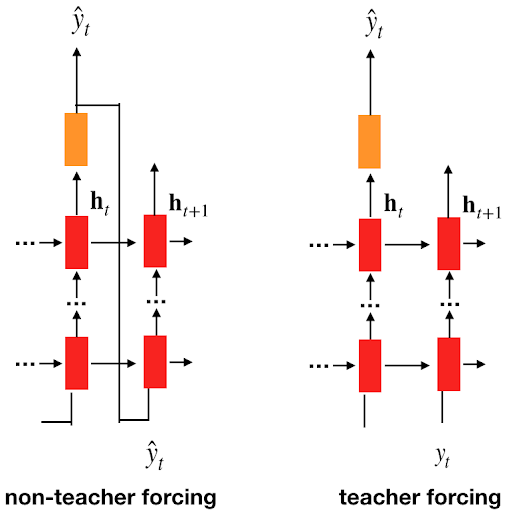
\includegraphics[width=0.4\linewidth]{images/teacher_forcing_teo.png}}
    \qquad \qquad
    \subfigure[Decoding comparison without and with teacher forcing, an example.]{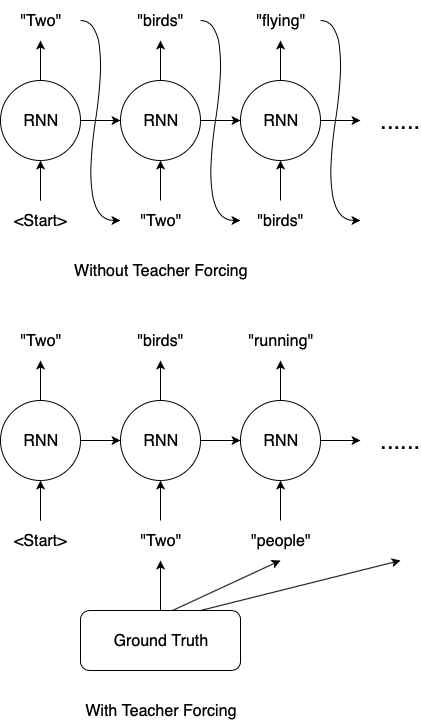
\includegraphics[width=0.28\linewidth]{images/teacher_forcing.png}}
    \caption{Teacher forcing technique, used only during the training phase.}
    \label{fig:teacher_forcing}
\end{figure}
We did fune-tuning on the encoders from Huggingface by training them together with the decoder, another solution that was tried by \cite{imamura-sumita-2019-recycling} suggested to freeze the encoder's weights and to train the decoder before a final training step where both layers would be trained at the same time, even though the paper stated that this would imply better performances from our models, we didn't find any major improvement on the SacreBLEU score.
\begin{comment}
\begin{listing}[H]
\begin{minted}[fontsize=\small, linenos, breaklines]{python}
def create_model(layers_size: int, num_layers: int, dense_size: int, num_heads: int, max_length: int, encoder=None) -> tf.keras.Model:
    # Encoder
    encoder_inputs = tf.keras.Input(shape=(None,), dtype="int32", name="encoder_inputs")
    if encoder is not None: 
        outputs = encoder(encoder_inputs)
        encoder_outputs = outputs.last_hidden_state
        layers_size = encoder_outputs.shape[-1]  # the size of the encoder and decoder layers must be the same
    else:
        encoder_outputs = EncoderTransformer(num_layers, layers_size, dense_size, num_heads, max_length, v_size_en)(encoder_inputs)

    # Decoder
    decoder_inputs = tf.keras.Input(shape=(None,), dtype="int32", name="decoder_inputs")
    encoded_seq_inputs = tf.keras.Input(shape=(None, layers_size), name="decoder_state_inputs")
    decoder_outputs = DecoderTransformer(num_layers, layers_size, dense_size, num_heads, max_length, v_size_it)(decoder_inputs, encoded_seq_inputs)
    decoder_outputs = layers.Dense(v_size_it, activation="softmax")(decoder_outputs)
    decoder = tf.keras.Model([decoder_inputs, encoded_seq_inputs], decoder_outputs, name="decoder_transformer")

    # Final model
    decoder_outputs = decoder([decoder_inputs, encoder_outputs])
    transformer = tf.keras.Model([encoder_inputs, decoder_inputs], decoder_outputs, name="transformer")
    return transformer
\end{minted}
\caption{Code to build our transformer model for translation.}
\label{lst:model_creation}
\end{listing}
\end{comment}
\subsection{Translator}\label{subsec:translator}
The translator class implements the method to translate a sentence, it takes as input a sentence to translate and returns it translated. The method works in this way: it tokenizes the sentence using the encoder tokenizer and gives it as input to the encoder. The decoder receives as input the start of sequence token ("[CLS]") then, at each time step $t$, it predicts the next token taking as input the one generated at the previous time step ($t-1$). This procedure is the same as the one shown in figure \ref{fig:teacher_forcing}, without taking into account the teacher forcing. We implemented several different ways to translate a sentence and the results are shown in \autoref{sec:results}.

\paragraph{Greedy search} Greedy search simply selects the word with the highest probability as its next word: $w_t = argmax_{w}P(w | w_{1:t-1})$ at each time step $t$. As sketched in figure \ref{fig:greedy_beam_search} \subref{fig:greedy_search}, starting from the word "The", the algorithm greedily chooses the next word of highest probability "nice" and so on, so that the final generated word sequence is ("The","nice","woman") having an overall probability of $0.5 \times 0.4=0.2$. This process can be visualized in figure \ref{fig:greedy_beam_search} \subref{fig:greedy_search}.

\paragraph{Beam search} Beam search reduces the risk of missing hidden high probability word sequences by keeping the most likely number of beams of hypotheses at each time step and eventually choosing the hypothesis that has the overall highest probability. Let's illustrate with num\_beams=2 in figure \ref{fig:greedy_beam_search} \subref{fig:beam_search}.

\begin{figure}[H]
\centering
\subfigure[Greedy search \label{fig:greedy_search}]%
{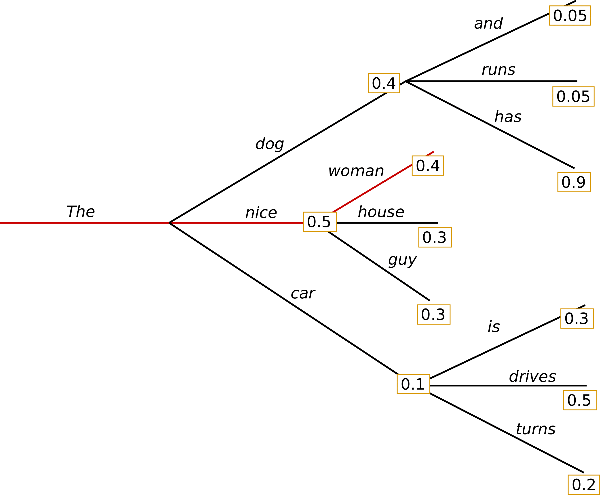
\includegraphics[width=0.47\linewidth]{images/greedy_search.png}} \qquad
\subfigure[Beam search \label{fig:beam_search}]%
{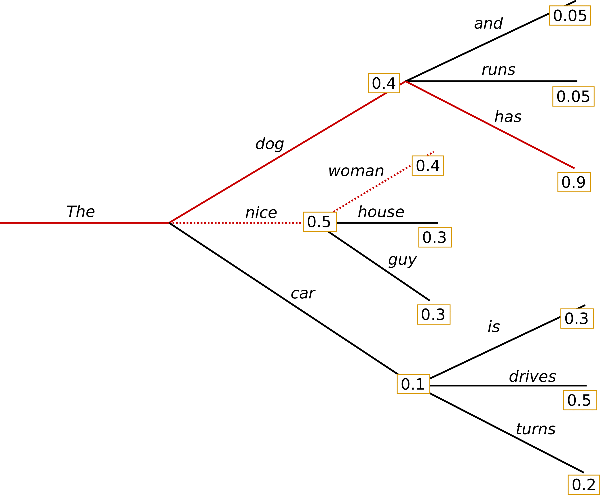
\includegraphics[width=0.47\linewidth]{images/beam_search.png}}
\caption{A comparison between greedy and beam search. \label{fig:greedy_beam_search}}
\end{figure}

\paragraph{Top-K sampling}
Beam search can work very well in tasks where the length of the desired generation is more or less predictable as in machine translation or summarization (\cite{yang2018breaking}). As argued in \cite{holtzman2019curious}, high quality human language does not follow a distribution of high probability next words. In other words, as humans, we want generated text to surprise us and not to be boring/predictable. The authors show this nicely by plotting the probability that a model would give to human text vs. what beam search does.

\begin{figure}[H]
    \centering
    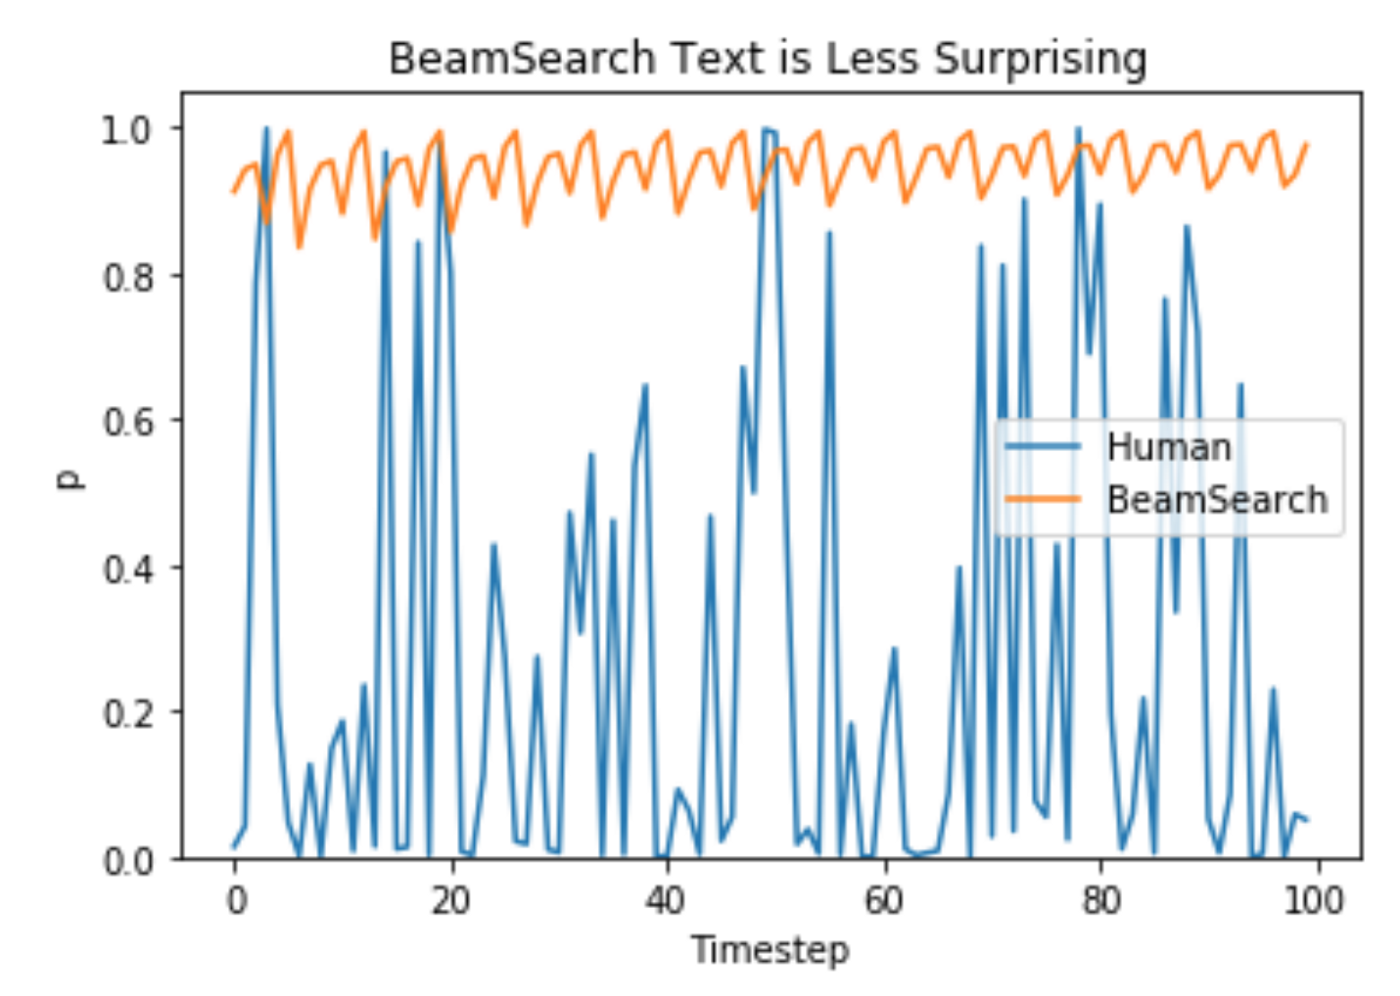
\includegraphics[width = .68\linewidth]{images/beam_search_vs_top_k_sampling.png}
    \caption{Beam search versus sampling approach.}
    \label{fig:beam_search_vs_sampling}
\end{figure}

\cite{fan2018hierarchical} introduced a simple, but very powerful sampling scheme, called Top-K sampling. In Top-K sampling, the K most likely next words are filtered and the probability mass is redistributed among only those K next words, this approach worked well in model for text generation like GPT2, and we know that is the field for which it was designed, anyway we wanted to test how this technique performs in machine translation. Whether a model is trained using a large dataset, we expect to have translations that differ each of other by some words, which are actually synonymous.

\begin{figure}[H]
    \centering
    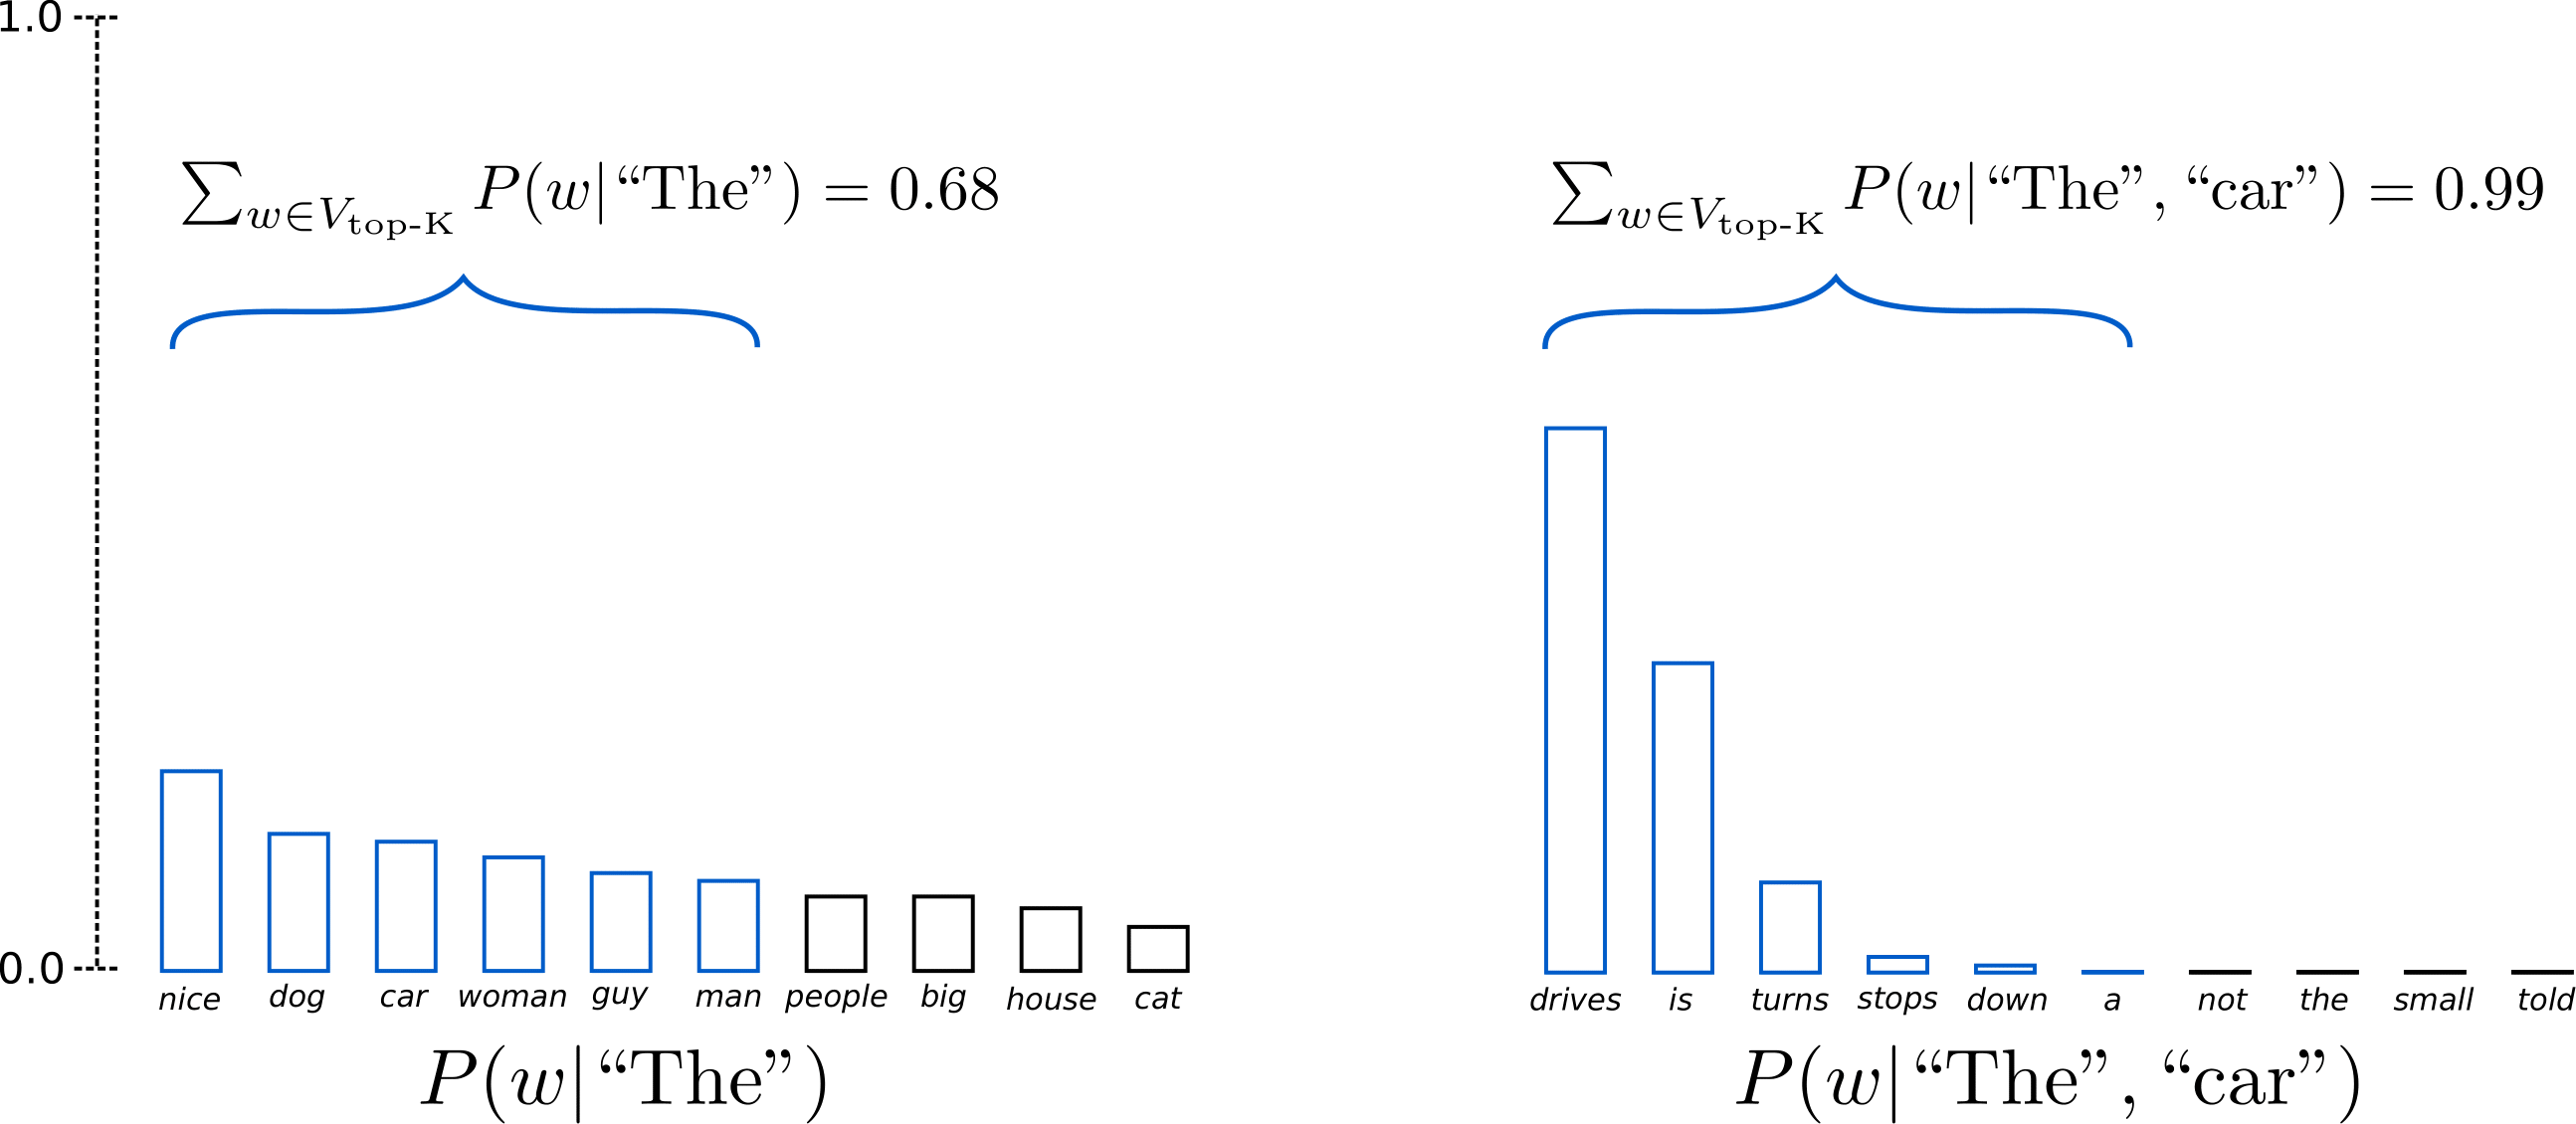
\includegraphics[width = .89\linewidth]{images/top_k_sampling.png}
    \caption{Top-k sampling approach.}
    \label{fig:topk_sampling}
\end{figure}

\subsection{Evaluation}
As we said at the end of section \ref{sec:dataset}, we used the Flores dataset by \cite{goyal2021flores} provided by Facebook as benchmark for our models, to evaluate the performances we need to translate the 1012 sentences in the set with each one of our trained models. We saved the translations on files which are then fed to a command that computes the sacreBLEU score as the guide from the Flores github suggests.
\begin{minted}[fontsize=\small, breaklines]{bash}
# Setup the benchmark by cloning the repository
!git clone --single-branch --branch adding_spm_tokenized_bleu https://github.com/ngoyal2707/sacrebleu.git
!python setup.py install

# Evaluate the model's translations by computing the BLEU score
!cat translation.txt | sacrebleu -tok spm flores101_dataset/devtest/ita.devtest
\end{minted}
We decided to evaluate our models on their translation with both top-k-sampling with k=1 (greedy search) and with k=5, even though the beam search works pretty well (there some examples in section \ref{app:beam_search}) it's too time consuming as it depends heavily on a sentence length and since the Flores dataset contains sentences that are long (we're talking about an average of 40 words per sentence) the beam search can take more then twenty times with respect to the other two approaches, so we decided to use it only for single cases.
